\documentclass{article}

\usepackage{pandekten}
\usepackage{dashrule}

\makeatletter
\newcommand*{\shifttext}[1]{%
  \settowidth{\@tempdima}{#1}%
  \hspace{-\@tempdima}#1%
}
\newcommand{\plabel}[1]{%
\shifttext{\textbf{#1}\quad}%
}
\newcommand{\prule}{%
\begin{center}%
\hdashrule[0.5ex]{.99\linewidth}{1pt}{1pt 2.5pt}%
\end{center}%
}

\makeatother

\newcommand{\minusbaseline}{\abovedisplayskip=0pt\abovedisplayshortskip=0pt~\vspace*{-\baselineskip}}%

\setlength{\parindent}{0pt}

\title{Assignment 11}
\author{Ze Chen}

\begin{document}

\maketitle

\plabel{1}%
The Lagrangian is given by
\begin{align*}
    \mathcal{L} &= \frac{1}{2}(\partial_\mu \sigma)^2 - \frac{1}{2}(2\mu^2)\sigma^2 + \frac{1}{2}(\partial_\mu \pi)^2 + \overline{\psi}\qty(i\slashed{\partial} - \frac{g\mu}{\sqrt{\lambda}}) \psi \\
    &\phantom{{}={}} - \sqrt{\lambda}\mu\sigma^3 - \sqrt{\lambda}\mu\sigma \pi^2 - \frac{\lambda}{4}\sigma^4 - \frac{\lambda}{2} \sigma^2 \pi^2 - \frac{\lambda}{4}\pi^4 - g\overline{\psi}(\sigma + i\gamma^5 \pi) \psi.
\end{align*}
The Feynman rules are listed below.
\begin{itemize}
  \item Vertices:
  \begin{center}
    
\includegraphics{img/yukawa/broken/vertex/vertex.pdf}
  \end{center}
  \item Propagators:
  \begin{center}
    
\includegraphics{img/yukawa/broken/propagator/propagator.pdf}
  \end{center}
\end{itemize}
\plabel{(b)}%
The tree level diagrams for $\psi(p_1,s_1)+\overline{\psi}(p_2,s_2)\rightarrow \psi(p_3,s_3)+\overline{\psi}(p_4,s_4)$ are given below.
\begin{center}
    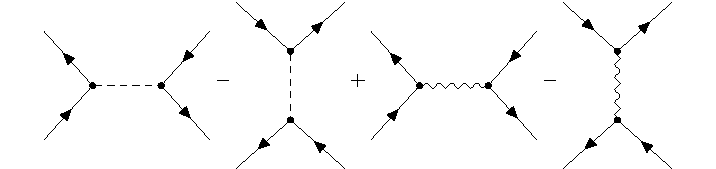
\includegraphics{img/yukawa/bhabha/bhabha.pdf}
\end{center}
Let $u_1 = u(p_1,s_1)$, $\overline{v}_2 = \overline{v}(p_2,s_2)$, $\overline{u}_3 = \overline{u}(p_3,s_3)$, and $v_4 = v(p_4, s_4)$, then
\begin{align*}
    i\mathcal{M} &= (-ig)^2 \biggl[ \overline{u}_3 u_1 \frac{i}{t - m^2_\sigma} \overline{v}_2 v_4 + \overline{u}_3 i\gamma^5 u_1 \frac{i}{t} \overline{v}_2 i\gamma^5 v_4 \\
    &\phantom{{}={}(-ig)^2\biggl[} - \overline{v}_2 u_1 \frac{i}{s-m_\sigma^2} \overline{u}_3 v_4 - \overline{v}_2 i\gamma^5 u_1 \frac{i}{s} \overline{u}_3 i\gamma^5 v_4 \biggr].
\end{align*}
It's clear that $i\mathcal{M}$ has a singularity when $s = m_\sigma^2$.

\plabel{(c)}%
The propagator is given by (for $x^0>y^0$)
\begin{align*}
    G(x-y) &= \int \frac{\dd[4]{p}}{(2\pi)^4} \frac{i}{p^2 - m_\sigma^2 + i\Gamma m_\sigma} e^{-ip\cdot(x-y)} \\
    &= \int \frac{\dd[4]{p}}{(2\pi)^4} \frac{i}{2E_{\vb{p}}(p^0 - E_{\vb{p}}+i(m/E_{\vb{p}})\Gamma/2)} e^{-ip\cdot(x-y)} \\
    &= \int \frac{\dd[3]{\vb{p}}}{(2\pi)^3} \frac{-1}{2 E_{\vb{p}}} e^{-ip\cdot (x-y)} \exp{-(m/E_{\vb{p}})\Gamma/2 (x^0 - y^0)} \\
    &\approx e^{-\Gamma/2 (x^0 - y^0)} G_0(x-y).
\end{align*}

\plabel{(d)}%
For $s$ close to $m_\sigma^2$,
\begin{align*}
    i\mathcal{M} &\approx (-ig)^2\qty(-\overline{v}_2 u_1 \frac{i}{s - m_\sigma^2 + i\Gamma m_\sigma} \overline{u}_3 v_4), \\
    \abs{\mathcal{M}}^2 &\propto \frac{1}{(s-m_\sigma^2)^2 + \Gamma^2 m_\sigma^2}.
\end{align*}
The width is given by $\Delta s = \Gamma m_\sigma$.

\plabel{(e)}%
The one-loop 1PI diagrams of $\sigma$ are listed below.
\begin{center}
    \begin{tabular}{m{4cm} m{3cm}}
        \centering
            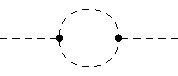
\includegraphics{img/yukawa/1pi/sigma-sigma/sigma-sigma.pdf}
         & $D=0$ \\
        \centering
            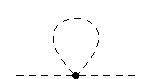
\includegraphics{img/yukawa/1pi/sigma-sigma/sigma2-sigma.pdf}
         & $D=-2$ \\
         \centering
            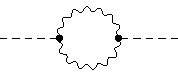
\includegraphics{img/yukawa/1pi/sigma-pi/sigma-pi.pdf}
         & $D=0$ \\
         \centering
            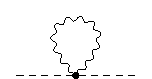
\includegraphics{img/yukawa/1pi/sigma-pi/sigma2-pi.pdf}
         & $D=-2$ \\
         \centering
            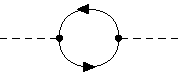
\includegraphics{img/yukawa/1pi/sigma-psi/sigma-psi.pdf}
         & $D=2$
    \end{tabular}
\end{center}
The counter term that cancels $\sigma$'s 1PI divergence is
\[ \delta \mathcal{L}_{\sigma\sigma} = \frac{\delta_Z}{2}(\partial_\mu \sigma)^2 - \frac{1}{2}(\delta_\mu + 3\delta_\lambda v^2) \sigma^2. \]
From the optical theorem we have
\[ \Gamma = -\frac{Z}{m_\sigma} \Im M^2(m_\sigma^2), \]
i.e.
\[ \Im M^2(m_\sigma^2) \propto -m_\sigma \Gamma \propto \lambda m^2_\sigma. \]

\plabel{(f)}%
The one-loop 1PI diagrams of $\psi$ are listed below.
\begin{center}
    \begin{tabular}{m{4cm} m{3cm}}
        \centering
            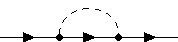
\includegraphics{img/yukawa/1pi/psi-sigma/psi-sigma.pdf}
         & $D=1$ \\
        \centering
            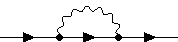
\includegraphics{img/yukawa/1pi/psi-pi/psi-pi.pdf}
         & $D=1$
    \end{tabular}
\end{center}
The one-loop 1PI diagrams of $\pi$ are listed below.
\begin{center}
    \begin{tabular}{m{4cm} m{3cm}}
        \centering
            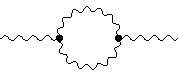
\includegraphics{img/yukawa/1pi/pi-pi/pi-pi.pdf}
         & $D=0$ \\
        \centering
            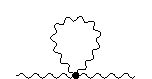
\includegraphics{img/yukawa/1pi/pi-pi/pi2-pi.pdf}
         & $D=-2$ \\
         \centering
            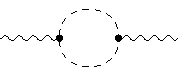
\includegraphics{img/yukawa/1pi/pi-sigma/pi-sigma.pdf}
         & $D=0$ \\
         \centering
            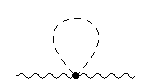
\includegraphics{img/yukawa/1pi/pi-sigma/pi2-sigma.pdf}
         & $D=-2$ \\
         \centering
            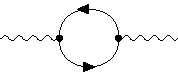
\includegraphics{img/yukawa/1pi/pi-psi/pi-psi.pdf}
         & $D=2$
    \end{tabular}
\end{center}
The counter terms in the Lagrangian before symmetry breaking are given by
\begin{align*}
    \delta \mathcal{L} &= \frac{1}{2} \delta_Z (\partial_\mu \phi^i)^2 - \frac{1}{2} \delta_\mu (\phi^i)^2 - \frac{\delta_\lambda}{4} ((\phi^i)^2)^2 \\
    &\phantom{{}={}} + i\overline{\psi} \delta_2 \slashed{\partial} \psi - \delta_1 g(\phi_1 + i\gamma^5) \psi.
\end{align*}
After symmetry breaking their forms are given below.
\begin{center}
    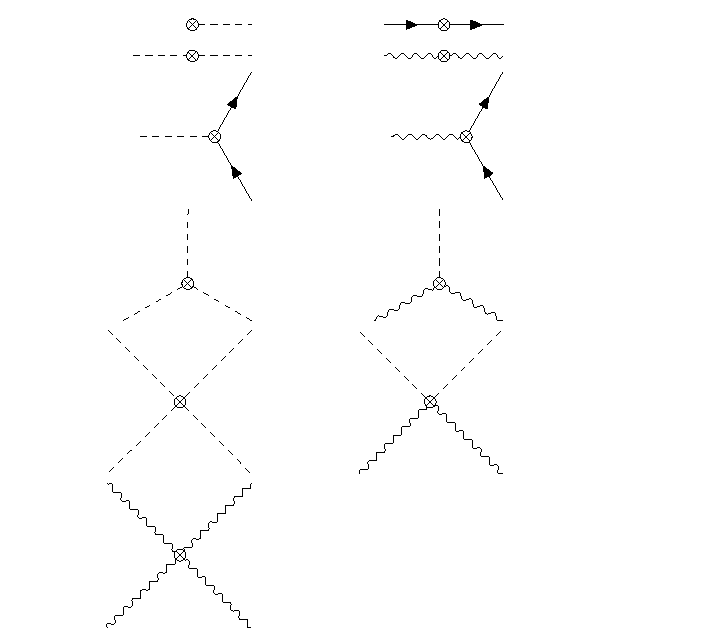
\includegraphics[width=.75\linewidth]{img/yukawa/counter/counter.pdf}
\end{center}
The renormalization conditions are given below.
\begin{center}
    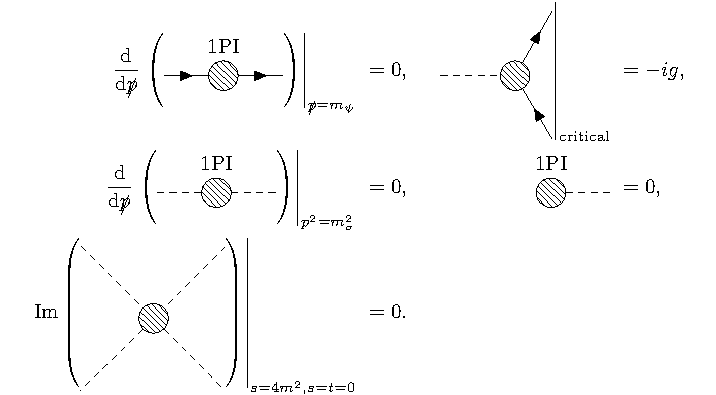
\includegraphics{img/yukawa/counter/rc.pdf}
\end{center}

\plabel{(g)}%
The Lagrangian get an extra EM term
\[ \mathcal{L}_{\mathrm{em}} = -\frac{1}{4}(F^{\mu\nu})^2 - e \overline{\psi} \slashed{A} \psi. \]
$\sigma$ may decay into photons via the following diagram.
\begin{center}
    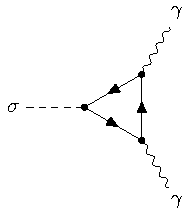
\includegraphics{img/yukawa/sigma-life/sigma-gamma-gamma.pdf}
\end{center}
For any parameters, $\sigma\rightarrow \pi+\pi$ could always happen.
The lowest order contribution to $\Im \Sigma_\sigma$ is the following diagram.
\begin{center}
    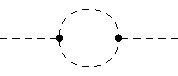
\includegraphics{img/yukawa/1pi/sigma-sigma/sigma-sigma.pdf}
\end{center}
The propagator in the loop may be replaced by the $\pi$.

\end{document}
